\documentclass[11pt,class=report,crop=false]{standalone}
\usepackage[screen]{../python}


\begin{document}


%====================================================================
\chapitre{Descente de gradient}
%====================================================================

\insertvideo{GE4UwT-JV4A}{partie 8.1. Descente de gradient classique}

\insertvideo{MJkY-E_0K74}{partie 8.2. Descente de gradients : exemples}

\insertvideo{HmAH6Ct1rc4}{partie 8.3. Descente de gradient et régression linéaire}

\insertvideo{4owcCc6iUiI}{partie 8.4. Descente de gradient stochastique}

\insertvideo{uBzn5sVtRzY}{partie 8.5. Accélération de la descente de gradient}




\objectifs{L'objectif de la méthode de descente de gradient est de trouver un minimum d'une fonction de plusieurs variables le plus rapidement possible. L'idée est très simple, on sait que le vecteur opposé au gradient indique une direction vers des plus petites valeurs de la fonction, il suffit donc de suivre d'un pas cette direction et de recommencer. Cependant, afin d'être encore plus rapide, il est possible d'ajouter plusieurs paramètres qui demandent pas mal d'ingénierie pour être bien choisis.}

\index{gradient}
\index{descente de gradient!classique}

%%%%%%%%%%%%%%%%%%%%%%%%%%%%%%%%%%%%%%%%%%%%%%%%%%%%%%%%%%%%%%%%%%%%%
\section{Descente de gradient classique}


Imaginons une goutte d'eau en haut d'une colline. La goutte d'eau descend en suivant la ligne de plus grande pente et elle s’arrête lorsqu'elle atteint un point bas. C'est exactement ce que fait la descente de gradient : partant d'un point sur une surface, on cherche la pente la plus grande en calculant le gradient et on descend d'un petit pas, on recommence à partir du nouveau point jusqu'à atteindre un minimum local.

\begin{center}
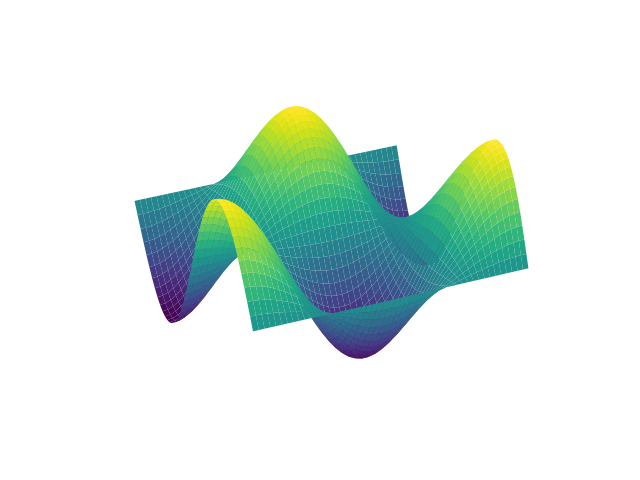
\includegraphics[scale=\myscale,scale=0.6]{figures/descente_intro}
\end{center}


%--------------------------------------------------------------------
\subsection{Où est le minimum ?}

On nous donne une fonction $f$ de deux variables $(a,b)$ et nous cherchons un point
$(a_{\min},b_{\min})$ en lequel $f$ atteint un minimum.
Voici la méthode expliquée par des dessins sur lesquels ont été tracées des lignes de niveau.

\begin{center}
\begin{minipage}{0.48\textwidth}
\begin{center}
{\bf (a) Au départ : rien}
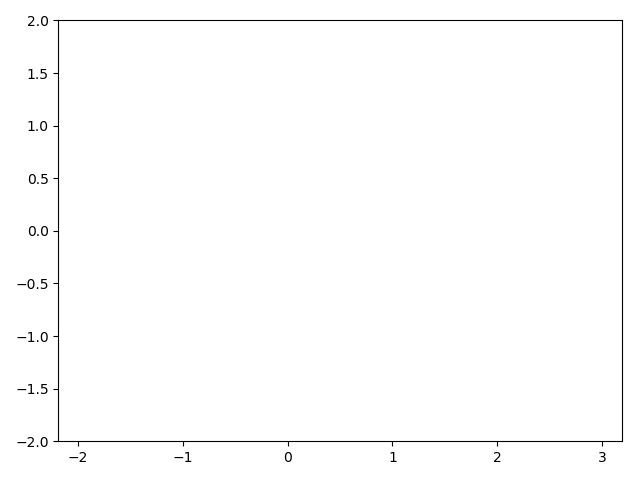
\includegraphics[scale=\myscale,scale=0.5]{figures/descente_intro_01}
\end{center}
\end{minipage}
\begin{minipage}{0.48\textwidth}
\begin{center}
{\bf (b) On part d'un point au hasard}
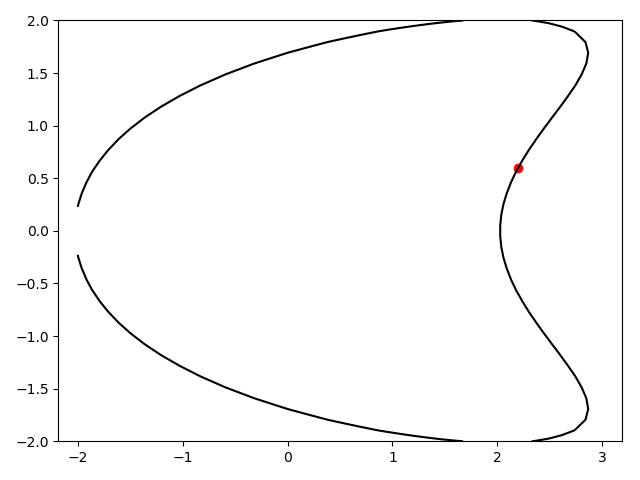
\includegraphics[scale=\myscale,scale=0.5]{figures/descente_intro_02}
\end{center}
\end{minipage}
\end{center}

\begin{center}
\begin{minipage}{0.48\textwidth}
\begin{center}
{\bf (c) On suit l'opposé du gradient}
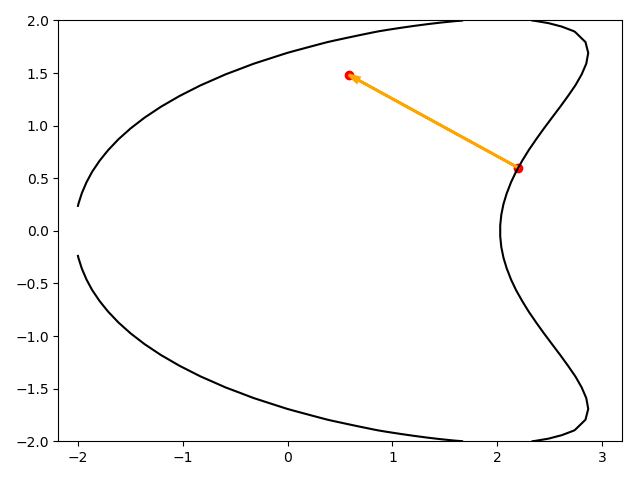
\includegraphics[scale=\myscale,scale=0.5]{figures/descente_intro_03}
\end{center}
\end{minipage}
\begin{minipage}{0.48\textwidth}
\begin{center}
{\bf (d) Depuis le nouveau point, on suit l'opposé du gradient}
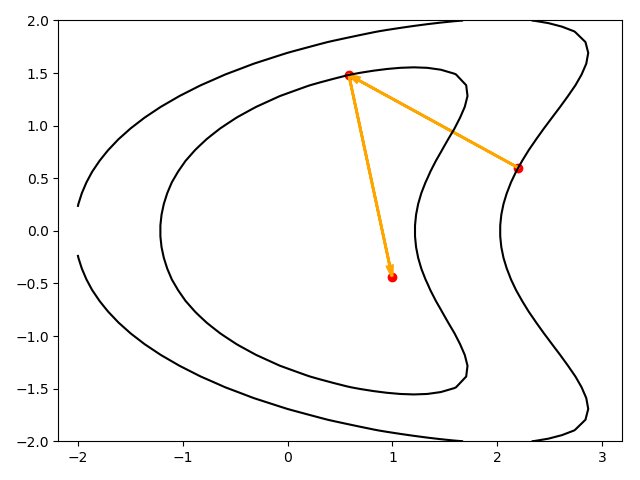
\includegraphics[scale=\myscale,scale=0.5]{figures/descente_intro_04}
\end{center}
\end{minipage}
\end{center}

\begin{center}
\begin{minipage}{0.48\textwidth}
\begin{center}
{\bf (e) On répète le processus}
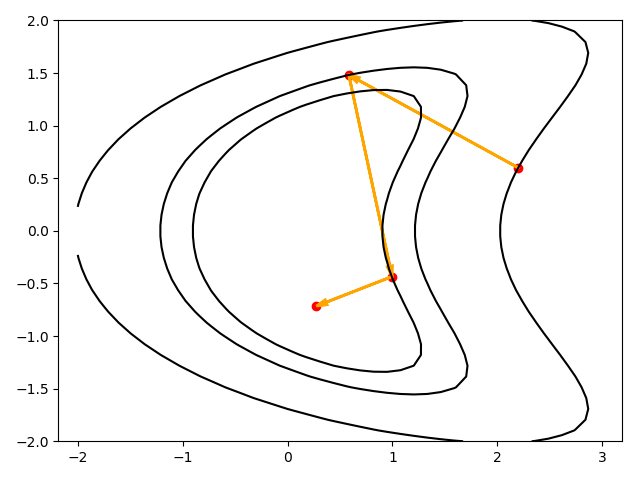
\includegraphics[scale=\myscale,scale=0.5]{figures/descente_intro_05}
\end{center}
\end{minipage}
\begin{minipage}{0.48\textwidth}
\begin{center}
{\bf (f) La suite converge vers le minimum}
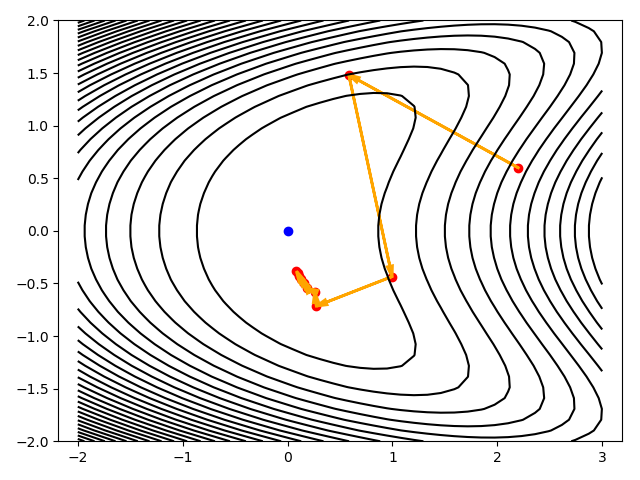
\includegraphics[scale=\myscale,scale=0.5]{figures/descente_intro_06}
\end{center}
\end{minipage}
\end{center}

{\bf Figure (a).} Au départ nous n'avons aucune information globale sur $f$. La seule opération que l'on s'autorise c'est calculer $\grad f(a,b)$ en certains points.

{\bf Figure (b).} On choisit un point $(a_0,b_0)$ au hasard. Si on note $c_0 = f(a_0,b_0)$ la valeur de $f$ en ce point, on sait que la ligne de niveau $(f=c_0)$ passe par $(a_0,b_0)$.

{\bf Figure (c).} On calcule en ce point le gradient de $f$. On trace l'opposé du gradient : $-\grad f(a_0,b_0)$. On sait d'une part que la ligne de niveau est orthogonale à ce gradient et surtout que dans la direction de $-\grad f(a_0,b_0)$, les valeurs de $f$ vont diminuer.

\myfigure{0.8}{
\tikzinput{fig-intro-01}
}

On se dirige alors dans la direction opposée au gradient d'un facteur $\delta$ (par exemple $\delta=0.1$). On arrive à un point noté $(a_1,b_1)$. Par construction, si $\delta$ est assez petit, la valeur $c_1 = f(a_1,b_1)$ est plus petite que $c_0$.

{\bf Figure (d).} On recommence depuis $(a_1,b_1)$. On calcule l'opposé du gradient en $(a_1,b_1)$, on se dirige dans cette nouvelle direction pour obtenir un point $(a_2,b_2)$ où $c_2 = f(a_2,b_2) < c_1$. 

{\bf Figure (e).} On itère le processus pour obtenir une suite de points $(a_k,b_k)$ pour lesquels $f$ prend des valeurs de plus en plus petites. 

{\bf Figure (f).}
On choisit de s'arrêter (selon une condition préalablement établie) et on obtient une valeur approchée $(a_N,b_N)$ du point $(a_{\min},b_{\min})$ en lequel $f$ atteint son minimum. 


\'Evidemment avec la vision globale de la fonction, on se dit qu'on aurait pu choisir un point de départ plus près et que certaines directions choisies ne sont pas les meilleures. Mais souvenez-vous que l'algorithme est \og{}aveugle\fg{}, il ne calcule pas les valeurs de $f$ en les $(a_k,b_k)$ et n'a pas connaissance du comportement de $f$ au voisinage de ces points.



%--------------------------------------------------------------------
\subsection{Exemple en deux variables}

Prenons l'exemple de $f(a,b) = a^2 + 3b^2$ dont le minimum est bien évidemment atteint en $(0,0)$ et appliquons la méthode du gradient.

Nous aurons besoin de calculer la valeur du gradient en certains points par la formule :
$$\grad f(a,b) = \left(\frac{\partial f}{\partial a}(a,b),\frac{\partial f}{\partial b}(a,b)\right) = (2a,6b).$$

Tout d'abord, on part d'un point $(a_0,b_0) = (2,1)$ par exemple.
Même si nous n'en avons pas besoin pour notre construction, on a $f(a_0,b_0) = 7$.
On calcule $\grad f(a_0,b_0) = (4,6)$. On fixe le facteur $\delta = 0.2$. On se déplace dans la direction opposée à ce gradient :
$$(a_1,b_1) = (a_0,b_0) - \delta \grad f(a_0,b_0) = (2,1)-0.2(4,6) = (2,1)-(0.8,1.2) = (1.2, -0.2).$$
On note que $f(a_1,b_1) = 1.56$ est bien plus petit que $f(a_0,b_0)$.
On recommence ensuite depuis $(a_1,b_1)$.
En quelques étapes les valeurs de $f$ tendent vers la valeur minimale et, dans notre cas, la suite converge vers $(0,0)$ (les valeurs sont approchées).

$$
\begin{array}{c|c|c|c}
k & (a_k,b_k) & \grad f(a_k,b_k) & f(a_k,b_k) \\ \hline
0 & (2, 1) & (4, 6) & 7 \\
1 & (1.2, -0.2) & (2.4, -1.20) & 1.56 \\
2 & (0.72, 0.04) & (1.44, 0.24) & 0.523 \\
3 & (0.432, -0.008) & (0.864, -0.048) & 0.186 \\
4 & (0.2592, 0.0016) & (0.5184, 0.0096) & 0.067 \\
5 & (0.15552, -0.00032) & (0.31104, -0.00192) & 0.024 \\
\cdots & & & \\
10 & (0.012, 1.02 \cdot 10^{-7}) & (0.024, 6.14\cdot 10^{-7}) & 0.00014 \\
\cdots &  & & \\
20 & (7.31\cdot 10^{-5}, 1.04 \cdot 10^{-14}) & (1.46 \cdot 10^{-4}, 6.29 \cdot 10 ^{-14}) & 5.34 \cdot 10^{-9} \\
\end{array}
$$

\bigskip

Voici les graphiques des premières itérations :
\begin{center}
\begin{minipage}{0.32\textwidth}
\begin{center}
{\bf Point initial}
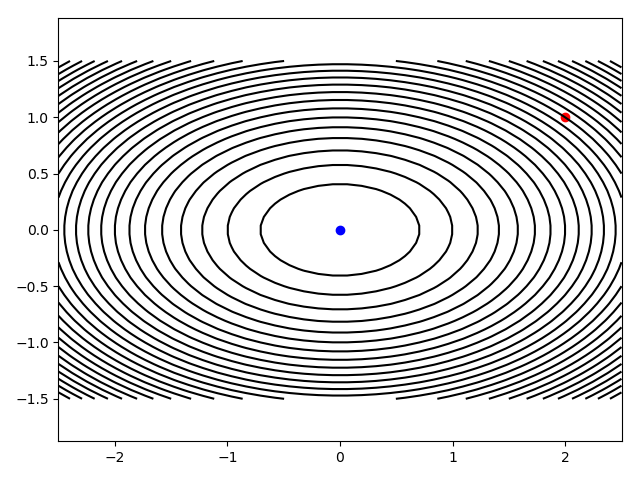
\includegraphics[scale=\myscale,scale=0.33]{figures/descente_deux_var_01}
\end{center}
\end{minipage}
\begin{minipage}{0.32\textwidth}
\begin{center}
{\bf Une itération}
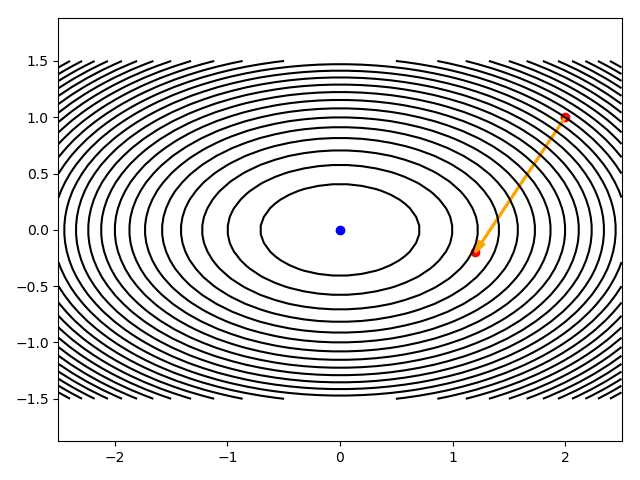
\includegraphics[scale=\myscale,scale=0.33]{figures/descente_deux_var_02}
\end{center}
\end{minipage}
\begin{minipage}{0.32\textwidth}
\begin{center}
{\bf Deux itérations}
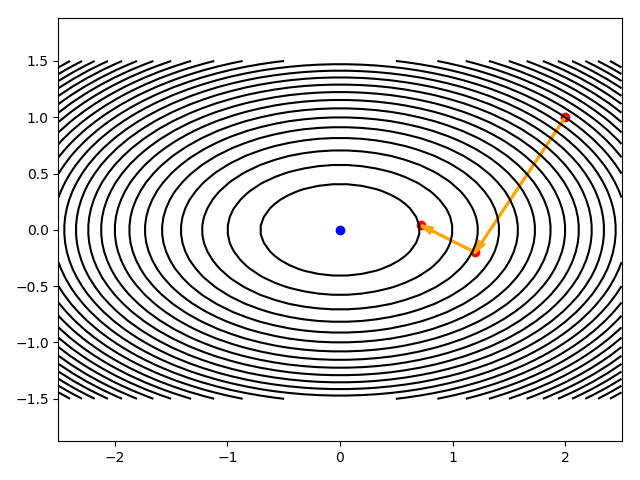
\includegraphics[scale=\myscale,scale=0.33]{figures/descente_deux_var_03}
\end{center}
\end{minipage}
\end{center}

\begin{center}
\begin{minipage}{0.32\textwidth}
\begin{center}
{\bf Trois itérations}
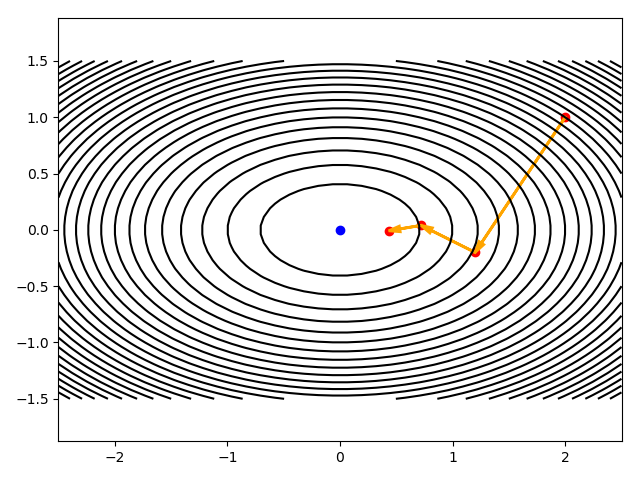
\includegraphics[scale=\myscale,scale=0.33]{figures/descente_deux_var_04}
\end{center}
\end{minipage}
\begin{minipage}{0.32\textwidth}
\begin{center}
{\bf Plus d'itérations}
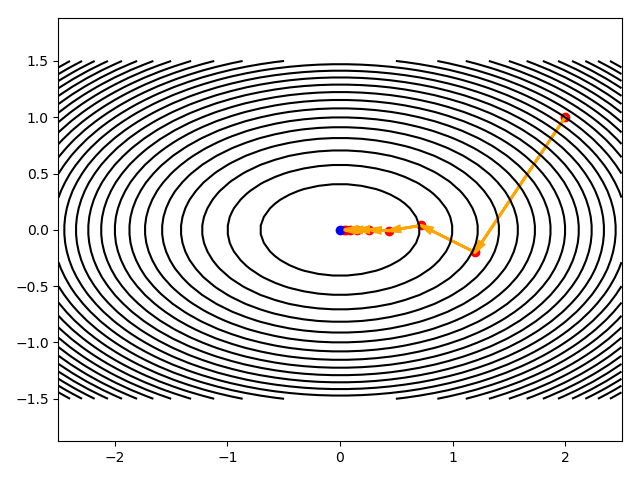
\includegraphics[scale=\myscale,scale=0.33]{figures/descente_deux_var_05}
\end{center}
\end{minipage}

\end{center}

Que se passe-t-il si l'on part d'un autre point ?
Partons cette fois de $(a_0,b_0) = (-1,-1)$ et fixons le pas à $\delta = 0.1$. 
Alors $(a_1,b_1)= (-0.8,-0.4)$, $(a_2,b_2) = (-0.64,-0.16)$\ldots{} 
La suite converge également vers $(0,0)$.
\begin{center}
  \begin{minipage}{0.45\textwidth}
    \begin{center}
      {\bf Partant de $(-1,-1)$ avec $\delta=0.1$}
      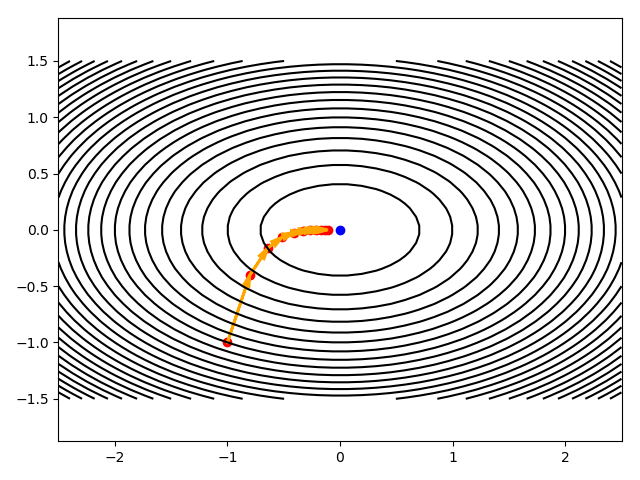
\includegraphics[scale=\myscale,scale=0.4]{figures/descente_deux_var_06}
    \end{center}
  \end{minipage}
\end{center}


%--------------------------------------------------------------------
\subsection{Exemples en une variable}

La descente de gradient fonctionne aussi très bien pour les fonctions d'une seule variable et sa visualisation est instructive.

\begin{exemple}
Considérons la fonction $f : \Rr \to \Rr$ définie par 
$$f(a) = a^2+1.$$
Il s'agit de trouver la valeur en laquelle $f$ atteint son minimum, c'est clairement $a_{\min}=0$ pour lequel $f(a_{\min})=1$. Retrouvons ceci par la descente de gradient.

Partant d'une valeur $a_0$ quelconque, la formule de récurrence est :
$$a_{k+1} = a_k - \delta \grad f(a)$$
où $\delta$ est le pas, choisi assez petit, et $\grad f(a) = f'(a) = 2a$.
Autrement dit :
$$a_{k+1} = a_k - 2 \delta a_k.$$

Voici le tableau des valeurs pour un pas $\delta=0.2$ et une valeur initiale $a_0=2$.

$$
\begin{array}{c|c|c|c}
k & a_k & f'(a_k) = \grad f(a_k) & f(a_k) \\ \hline
0 & 2 & 4 & 5 \\
1 & 1.2 & 2.4 & 2.44 \\
2 & 0.72 & 1.44 & 1.5184 \\
3 & 0.43 & 0.86 & 1.1866 \\
4 & 0.25 & 0.5184 & 1.0671 \\
5 & 0.15 & 0.31 & 1.0241 \\
6 & 0.093 & 0.186 & 1.0087 \\
7 & 0.055 & 0.111 & 1.0031 \\
8 & 0.033 & 0.067 & 1.0011 \\
9 & 0.020 & 0.040 & 1.0004 \\
10 & 0.012 & 0.024 & 1.0001 \\
\end{array}
$$

Voici la version graphique de ces $10$ premières itérations (figure de gauche).
Si l'on change le point initial, ($a_0=-1.5$ sur la figure de droite) alors la suite $(a_k)$ converge vers la même valeur $a_{\min}=0$.

\begin{center}
\begin{minipage}{0.48\textwidth}
\begin{center}
$\delta=0.2$ \quad $a_0=2$
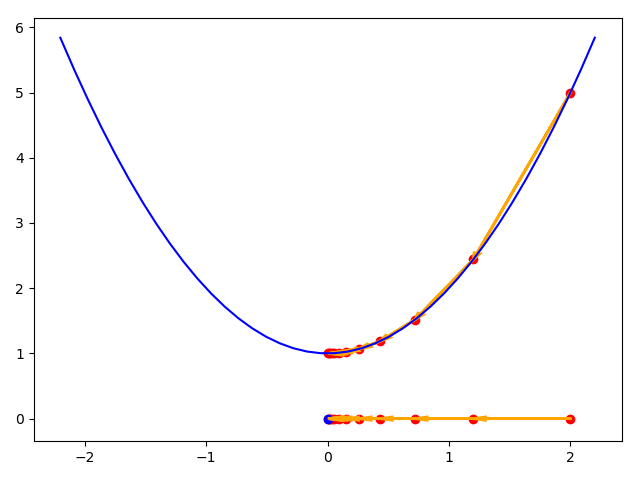
\includegraphics[scale=\myscale,scale=0.5]{figures/descente_une_var_01}
\end{center}
\end{minipage}
\begin{minipage}{0.48\textwidth}
\begin{center}
$\delta=0.2$ \quad $a_0=-1.5$
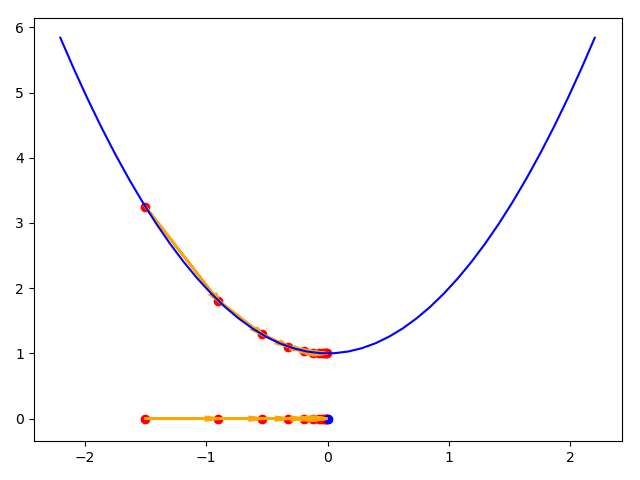
\includegraphics[scale=\myscale,scale=0.5]{figures/descente_une_var_02}
\end{center}
\end{minipage}
\end{center}

Il faut bien comprendre ce graphique : la suite des points $(a_k)$ \couleurnb{(points rouges) }{}se lit sur l'axe des abscisses. Les vecteurs \couleurnb{(orange) }{}montrent les itérations.
Il est plus facile de comprendre l'algorithme sur le graphe de $f$\couleurnb{ (en bleu)}{}. Sur ce graphe, on reporte les points $(a_k,f(a_k))$\couleurnb{ (en rouge)}{}, ce qui permet de bien comprendre que les valeurs $f(a_k)$ décroissent rapidement. On note aussi que le gradient (ici $f'(a_k)$) diminue à l'approche du minimum, ce qui se traduit par des vecteurs (c'est-à-dire l'écart entre deux points successifs) de plus en plus petits. 

\end{exemple}

Justifions l'algorithme et l'intervention du gradient dans le cas d'une variable.
Si la fonction est croissante sur un intervalle, $f'(a)>0$ pour tout $a$ dans cet intervalle et la formule
$$a_{k+1} = a_k - \delta f'(a_k) \quad \text{ donne } \quad a_{k+1}<a_k.$$
Ainsi $f(a_{k+1}) < f(a_k)$ et l'ordonnée du point $(a_{k+1},f(a_{k+1}))$ est donc inférieure à celle du point $(a_k,f(a_k))$.
Par contre, si $f$ est décroissante alors $f'(a)<0$ et
$$a_{k+1} = a_k - \delta f'(a_k) \quad \text{ donne } \quad a_{k+1}>a_k,$$
ce qui implique de nouveau $f(a_{k+1}) < f(a_k)$ (car $f$ est décroissante).

Dans tous les cas, l'ordonnée du point $(a_{k+1},f(a_{k+1}))$ est inférieure à celle du point $(a_k,f(a_k))$.

\myfigure{1}{
\tikzinput{fig_descente-02}
}

\begin{exemple}
Le choix du paramètre $\delta$ est important.
Reprenons la fonction $f$ définie par $f(x) = x^2+1$ et testons différentes \og{}mauvaises\fg{} valeurs du pas $\delta$ (avec toujours $a_0=2$).

\begin{center}
\begin{minipage}{0.32\textwidth}
\begin{center}
$\delta=0.9$
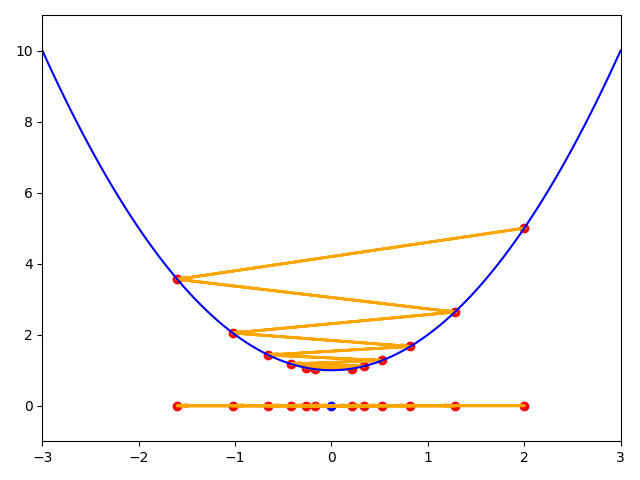
\includegraphics[scale=\myscale,scale=0.3]{figures/descente_une_var_03}
\end{center}
\end{minipage}
\begin{minipage}{0.32\textwidth}
\begin{center}
$\delta=1.1$
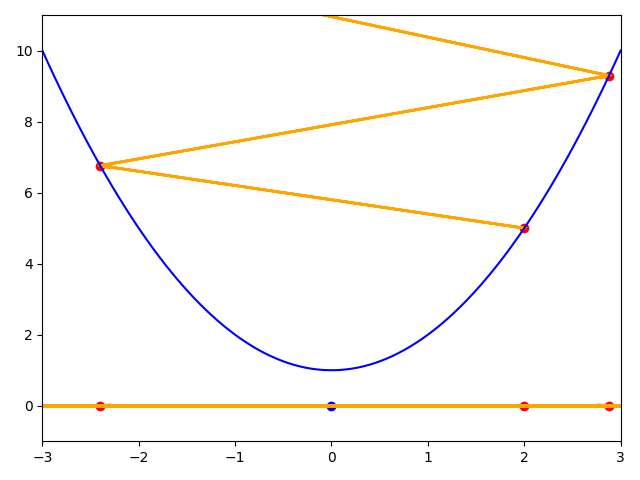
\includegraphics[scale=\myscale,scale=0.3]{figures/descente_une_var_04}
\end{center}
\end{minipage}
\begin{minipage}{0.32\textwidth}
\begin{center}
$\delta=0.05$
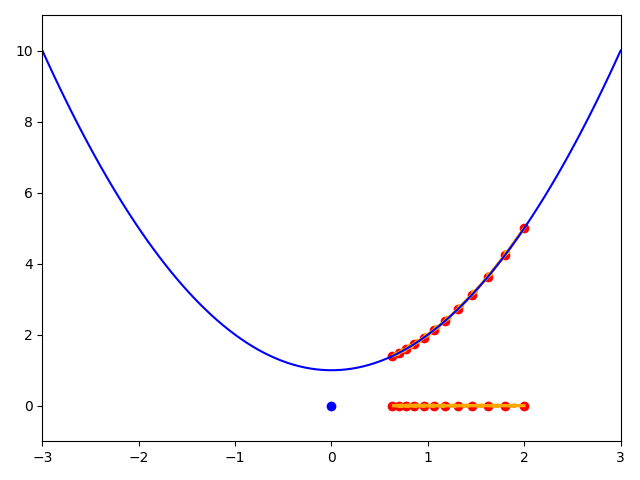
\includegraphics[scale=\myscale,scale=0.3]{figures/descente_une_var_05}
\end{center}
\end{minipage}
\end{center}

\begin{itemize}
  \item Pour $\delta = 0.9$, la suite $(a_k)$ tend bien vers $a_{\min} = 0$. Les ordonnées sont bien décroissantes mais comme $\delta$ est trop grand, la suite des points oscille de part et d'autre du minimum.
  
  \item Pour $\delta = 1.1$, la suite $(a_k)$ diverge. Les ordonnées augmentent, la suite des points oscille et s'échappe. Cette valeur de $\delta$ ne donne pas de convergence vers un minimum.
  
  \item Pour $\delta = 0.05$, la suite $(a_k)$ tend bien vers $a_{\min}$ mais, comme $\delta$ est trop petit, il faudrait beaucoup d'itérations pour arriver à une approximation raisonnable.
  
\end{itemize}
\end{exemple}

\begin{exemple}
Le choix du point de départ est également important surtout lorsqu'il existe plusieurs minimums locaux.
Soit la fonction $f$ définie par :
$$f(a) = a^4 -5a^2 + a + 10.$$
Cette fonction admet deux minimums locaux.
La suite $(a_k)$ de la descente de gradient converge vers l'un de ces deux minimums selon le choix du point initial $a_0$ (ici $\delta=0.02$).

\begin{center}
\begin{minipage}{0.48\textwidth}
\begin{center}
$a_0=-2$
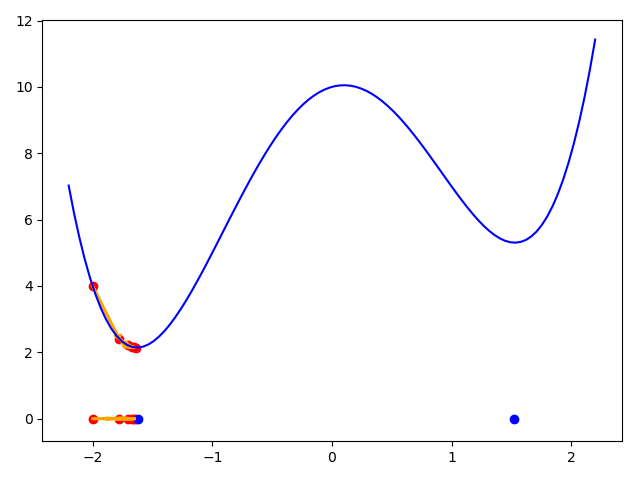
\includegraphics[scale=\myscale,scale=0.5]{figures/descente_une_var_06}
\end{center}
\end{minipage}
\begin{minipage}{0.48\textwidth}
\begin{center}
$a_0=-0.5$
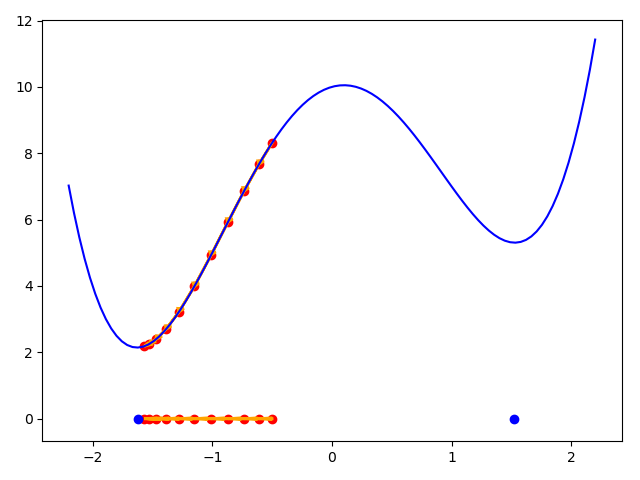
\includegraphics[scale=\myscale,scale=0.5]{figures/descente_une_var_07}
\end{center}
\end{minipage}

\bigskip

\begin{minipage}{0.48\textwidth}
\begin{center}
$a_0=0.5$
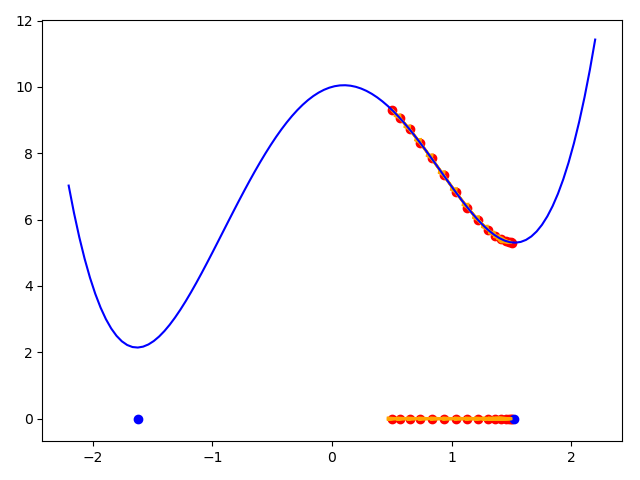
\includegraphics[scale=\myscale,scale=0.5]{figures/descente_une_var_08}
\end{center}
\end{minipage}
\begin{minipage}{0.48\textwidth}
\begin{center}
$a_0=2$
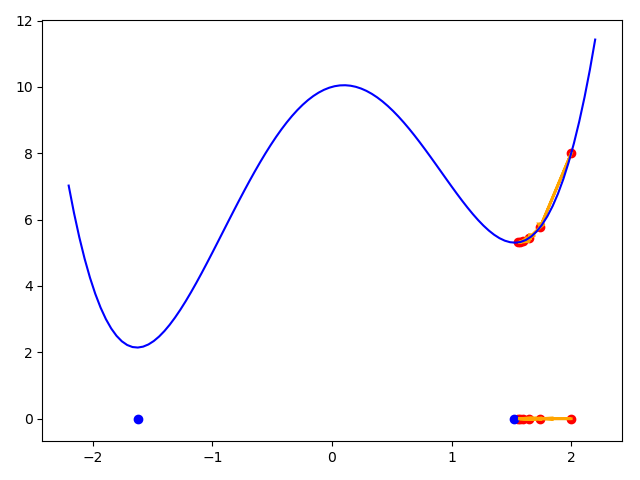
\includegraphics[scale=\myscale,scale=0.5]{figures/descente_une_var_09}
\end{center}
\end{minipage}
\end{center}
\end{exemple}


\begin{exemple}
Les points-selles posent également problème.

La fonction $f$ définie par 
$$f(a) = a^4-2a^3+4$$
a pour dérivée $f'(a) = 4a^3-6a^2$ qui s'annule en $a=0$ qui est l'abscisse d'un point-selle (ni un  minimum ni un maximum, en fait la fonction est strictement décroissante autour de $a=0$). La dérivée s'annule aussi en $a=\frac32$ où est atteint le minimum global.

Voici les $100$ premières itérations pour la descente de gradient en partant de $a_0=-1$ (avec $\delta = 0.05$) : la suite $a_k$ converge vers $0$ qui n'est pas le minimum recherché.

\begin{center}
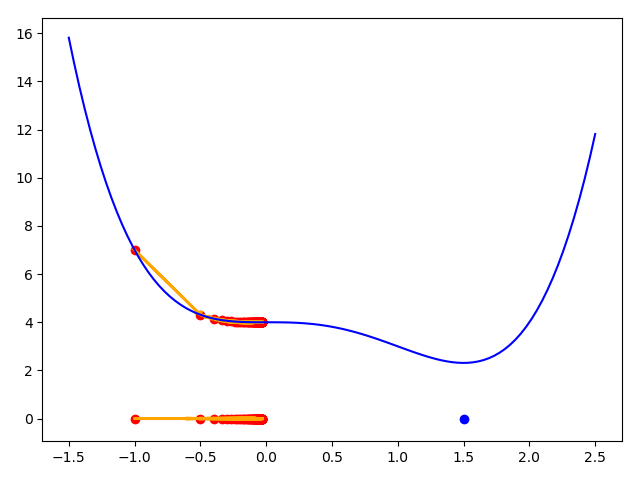
\includegraphics[scale=\myscale,scale=0.5]{figures/descente_une_var_10}
\end{center}
\end{exemple}

%--------------------------------------------------------------------
\subsection{Algorithme du gradient}

Formalisons un peu les choses pour mettre en évidence l'idée générale et les problèmes techniques qui surviennent.

\textbf{Algorithme de la descente de gradient.}


Soit une fonction $f : \Rr^n \to \Rr$, $P \mapsto f(P)$ de plusieurs variables, avec $P = (a_1,\ldots,a_n)$, dont on sait calculer le gradient $\grad f (P)$.

\textbf{Données.}
\begin{itemize}
  \item Un point initial $P_0 \in \Rr^n$.
  \item Un niveau d'erreur $\epsilon>0$. 
\end{itemize}

\textbf{Itération.}
On calcule une suite de points $P_1,P_2,\ldots \in \Rr^n$ par récurrence de la façon suivante. Supposons que l'on ait déjà obtenu le point $P_k$ :
\begin{itemize}
  \item on calcule $\grad f(P_k)$,
  \item on choisit un pas $\delta_k$ et on calcule
  $$P_{k+1} = P_k - \delta_k \grad f (P_k).$$
\end{itemize}  

\myfigure{1}{
\tikzinput{fig_descente-01}
}


\textbf{Arrêt.}
On s'arrête lorsque $\|\grad f(P_k) \| \le \epsilon$.


\bigskip

\begin{remarque*}
\sauteligne
\begin{itemize}
  \item \'Evidemment, plus on choisit le point initial $P_0$ proche d'un minimum local, plus l'algorithme va aboutir rapidement. Mais comme on ne sait pas où est ce minimum local (c'est ce que l'on cherche), le plus simple est de choisir un $P_0$ au hasard.

  \item Le choix du pas $\delta_k$ est crucial. On sait que l'on peut choisir $\delta_k$ assez petit de façon à avoir $f(P_{k+1}) \le f(P_k)$ car dans la direction de $-\grad f(P_k)$ la fonction $f$ décroît.
  
  \myfigure{1}{
  \tikzinput{fig_descente-03}
  }
  
  On peut fixer à l'avance un pas $\delta$ commun à toutes les itérations, par exemple $\delta = 0.01$. On pourrait également tester à chaque itération plusieurs valeurs de $\delta$ par balayage ($\delta = 0.001$, puis $\delta=0.002$\ldots) et choisir pour $\delta_k$ celui en lequel $f$ prend la plus petite valeur.
  
  \item Le critère d'arrêt assure qu'en $P_k$ le gradient est très petit. Cela ne garantit pas que ce point soit proche d'un minimum local (et encore moins d'un minimum global). Souvenez-vous : en un minimum local le gradient est nul, mais ce n'est pas parce que le gradient est nul que l'on a atteint un minimum local, cela pourrait être un point-selle voire un maximum local.
  
    Dans la pratique, on ne définira pas de seuil d'erreur $\epsilon$, mais un nombre d'itérations fixé à l'avance.
  
  \item Il est important de calculer $\grad f(a_1,\ldots,a_n)$ rapidement. On pourrait bien sûr calculer une approximation de chacune des dérivées partielles $\frac{\partial f}{\partial a_i}(a_1,\ldots,a_n)$ comme un limite. Mais pour gagner en temps et en précision, on préfère que ce calcul soit fait à l'aide de son expression exacte. 
  
\end{itemize}
\end{remarque*}



%%%%%%%%%%%%%%%%%%%%%%%%%%%%%%%%%%%%%%%%%%%%%%%%%%%%%%%%%%%%%%%%%%%%%
\section{Optimisation}

Nous allons d'une part résoudre des problèmes d'optimisation : quelle droite approche au mieux un nuage de points, et d'autre part étudier comment améliorer le choix du pas $\delta$.


%--------------------------------------------------------------------
\subsection{Faire varier le pas}

On se concentre d'abord sur le choix du \defi{pas}\index{descente de gradient!pas} $\delta$ (\emph{learning rate}).

Rappelons tout d'abord que lorsque l'on se rapproche d'un point minimum, le gradient tend vers $0$. Le vecteur $\delta \grad f(P_k)$ tend donc vers $0$ à l'approche du minimum, même si $\delta$ reste constant.

Cependant, il faut choisir $\delta$ ni trop grand, ni trop petit : $\delta$ ne doit pas être trop grand car sinon les points $P_k$ vont osciller autour du minimum, mais si $\delta$ est trop petit alors les points $P_k$ ne s'approcheront du minimum qu'au bout d'un temps très long. Une solution est de faire varier $\delta$. Pour les premières itérations, on choisit un $\delta_k$ assez grand, puis de plus en plus petit au fil des itérations.

Voici différentes formules possibles, à chaque fois $\delta_0$ est le pas initial (par exemple $\delta_0=0.1$ ou $\delta_0=0.01$).

\textbf{Décroissance linéaire.}
$$\delta_k = \frac{\delta_0}{k+1}.$$

\textbf{Décroissance quadratique.}
$$\delta_k = \frac{\delta_0}{(k+1)^2}.$$

\textbf{Décroissance exponentielle.}
$$\delta_k = \delta_0 e^{-\beta k}$$
où $\beta$ est une constante positive.


\textbf{Décroissance linéaire utilisée par \keras}
$$\delta_k = \frac{\delta_0}{\alpha k+1}$$
où $\alpha\ge0$ est une constante (appelée \emph{decay}).
Si $\alpha=0$ alors $\delta_k$ est constant (et vaut $\delta_0$).
L'usage courant est d'utiliser des valeurs de $\alpha$ entre $10^{-4}$ et $10^{-6}$.


Terminons par rappeler que le bon choix d'un $\delta$ ou des $\delta_k$ n'a rien d'évident, il s'obtient soit par test à la main, soit par des expérimentations automatiques, mais à chaque fois il doit être adapté à la situation.



%--------------------------------------------------------------------
\subsection{Régression linéaire $y=ax+b$}

\index{regression lineaire@régression linéaire}

On considère un ensemble de $N$ points $A_i = (x_i,y_i)$, $i=1,\ldots,N$.
L'objectif est de trouver l'équation $y=ax+b$ de la droite qui approche au mieux tous ces points. Précisons ce que veut dire \og{}approcher au mieux\fg{} : il s'agit de minimiser la somme des carrés des distances verticales entre les points et la droite.


\myfigure{1}{
\tikzinput{fig-regression-01}
}

La formule qui donne l'erreur est :
$$E(a,b) = \sum_{i=1}^{N}\big(y_i - (ax_i+b)\big)^2,$$
autrement dit 
$$E(a,b) = \big(y_1 - (ax_1+b)\big)^2 + \cdots + \big(y_N - (ax_N+b)\big)^2.$$

Remarquons que l'on a toujours $E(a,b)\ge0$. Si par exemple tous les points sont alignés, alors on peut trouver $a$ et $b$ tels que $E(a,b)=0$. Quand ce n'est pas le cas, on cherche $a$ et $b$ qui rendent $E(a,b)$ le plus petit possible.
Il s'agit donc bien ici de minimiser une fonction de deux variables (les variables sont $a$ et $b$).

Nous allons appliquer la méthode de la descente de gradient à la fonction $E(a,b)$. Pour cela nous aurons besoin de calculer son gradient :
$$\grad E(a,b) 
= \left(\frac{\partial E}{\partial a}(a,b), \frac{\partial E}{\partial b}(a,b)\right)
= \left(
\sum_{i=1}^{N} -2x_i\big(y_i - (ax_i+b)\big),  
\sum_{i=1}^{N} -2\big(y_i - (ax_i+b)\big)
\right).$$


\begin{exemple}
Prenons d'abord l'exemple de trois points $A_1 = (0,3)$, $A_2 = (2,4)$ et $A_3 = (6,6)$ qui sont alignés. 

\myfigure{1}{
\tikzinput{fig-regression-02}
}

La fonction $E(a,b)$ s'écrit :
$$E(a,b) = (3-b)^2 + (4-(2a+b))^2 + (6-(6a+b))^2.$$
Partons arbitrairement de $(a_0,b_0) = (0,1)$ (qui correspond à la droite horizontale d'équation $y=1$).
Voici les valeurs successives $(a_k,b_k)$ obtenues par la méthode de descente de gradient pour un pas $\delta = 0.02$.

$$
\begin{array}{c|c|c|c}
k & (a_k,b_k) & \grad E(a_k,b_k) & E(a_k,b_k) \\ \hline
0 & (0, 1) & (-72 -20) &  38 \\
1 & (1.44, 1.4) & (49.60, 5.44) &  18.96 \\
2 & (0.44, 1.29) & (-31.50, -11.08) & 10.28 \\
3 & (1.07, 1.51) & (22.44, 0.32) &  6.24 \\
4 & (0.62, 1.50) & (-13.57, -6.89) &  4.27 \\
5 & (0.90, 1.64) & (10.35, -1.72) &  3.24 \\
\end{array}
$$

\smallskip

Au bout de $100$ itérations, on obtient $a_{100} \simeq 0.501$ et $b_{100} \simeq 2.99$ (avec un gradient et une erreur presque nuls). C'est bien la droite $y = \frac12x+3$ qui passe par les trois points.


Sur la figure de gauche ci-dessous, sont dessinés, dans le plan de coordonnées $(a,b)$, les premiers points $(a_k,b_k)$ qui convergent (lentement et en oscillant) vers $(\frac12,3)$\couleurnb{ (point bleu)}{}. Sur la figure de droite sont tracées, dans le plan de coordonnées $(x,y)$, les droites d'équation $y = a_kx+b_k$ pour les premières valeurs de $k$. 
Il est beaucoup plus difficile d'appréhender la convergence des droites (vers la droite d'équation $y=\frac12x+3$\couleurnb{ en bleu}{}) que celle des points de la figure de gauche.

\begin{center}
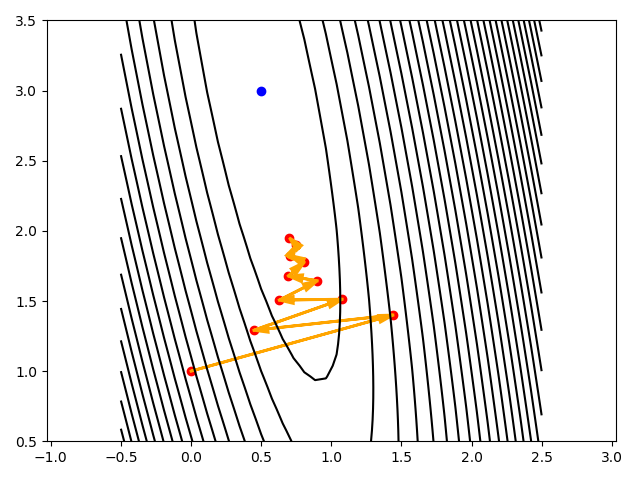
\includegraphics[scale=\myscale,scale=0.5]{figures/regression-01}
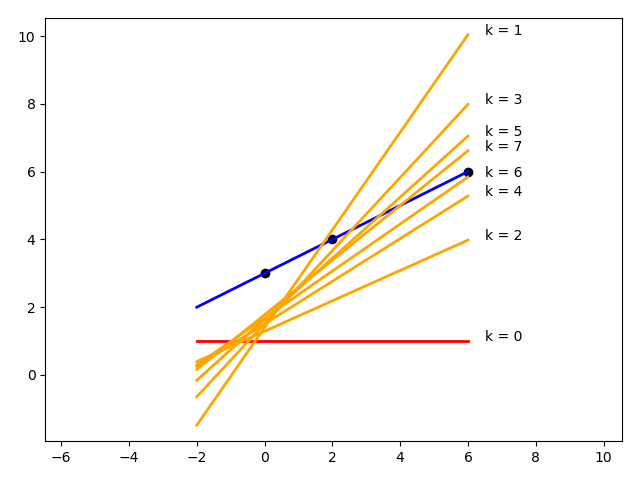
\includegraphics[scale=\myscale,scale=0.5]{figures/regression-02}
\end{center}
\end{exemple}

\begin{exemple}
\`A partir des données des $5$ points suivants, quelle ordonnée peut-on extrapoler pour le point d'abscisse $x=6$ ?

$$A_1 = (4,1),\quad A_2 = (7,3),\quad A_3 = (8,3),\quad A_4 = (10,6),\quad A_5 = (12,7).$$
\myfigure{0.5}{
\tikzinput{fig-regression-03}
}

Ces $5$ points sont à peu près alignés. On calcule la meilleure droite de régression linéaire par la descente de gradient. Cela revient par exemple à minimiser la fonction $E(a,b)$ présentée ci-dessus, mais actualisée avec nos données. 
On fixe un pas $\delta = 0.001$.
On ne choisit pas le point initial $(a_0,b_0)$ au hasard. Plus on part d'un point proche de la solution, plus la suite convergera rapidement. On trace la droite qui passe par le premier point $A_1$ et le dernier point $A_5$. Cette droite a pour équation $y=\frac34 x -2$ et est déjà une droite qui approche assez bien les $5$ points. Prenons cette droite comme point de départ, c'est-à-dire posons $(a_0,b_0) = (\frac34,-2)$.
La descente de gradient conduit au bout de $1000$ itérations à $a\simeq 0.78$ et $b\simeq -2.46$, pour l'équation de la droite de régression linéaire.

Sur le dessin ci-dessous sont tracées la droite initiale qui passe par les points $A_1$ et $A_5$ \couleurnb{(en rouge) }{}et la droite de régression linéaire\couleurnb{ (en bleu)}{}.

\myfigure{0.5}{
\tikzinput{fig-regression-04}
}

N'oublions pas de répondre à la question initiale. Selon notre modèle linéaire, pour $x=6$, on doit avoir $y=ax+b \simeq 2.22$ (le point $B$ de la figure ci-dessus).
\end{exemple}

Remarque : il existe une formule directe pour calculer exactement les coefficients $a$ et $b$ de la droite de régression linéaire, mais ce n'est pas l'esprit de ce cours.


%--------------------------------------------------------------------
\subsection{Régression linéaire et neurone}

Quel est le lien entre la régression linéaire et un neurone ?
En fait, le neurone suivant a pour fonction associée $F(x) = ax+b$.

\myfigure{1}{
\tikzinput{fig-regression-05}
}

Reformulons le problème de la régression linéaire ainsi : soit des données $(x_i,y_i)$, $i=1,\ldots,N$. Il s'agit de trouver pour le type de neurone choisi les coefficients $a$ et $b$, tels que la fonction $F$ associée au neurone réalise au mieux ces données, c'est-à-dire 
$$F(x_i) \simeq y_i.$$

Vocabulaire :
\begin{itemize}
  \item Chaque $x_i$ est une \defi{entrée},
  \item $y_i$ est la \defi{sortie attendue} pour l'entrée $x_i$,
  \item $F(x_i)$ est la \defi{sortie produite},
  \item $E_i = (y_i - F(x_i))^2$ est l'erreur pour l'entrée $x_i$,
  \item \defi{L'erreur totale} est $$E = \sum_{i=1}^N E_i =  \sum_{i=1}^N(y_i - F(x_i))^2.$$
  \item Vu que $F(x)=ax+b$, on retrouve bien pour $E$ la forme de la fonction présentée précédemment.
\end{itemize}


%--------------------------------------------------------------------
\subsection{Régression linéaire $z=ax+by+c$}

Le neurone suivant a pour fonction $F(x,y) = ax+by+c$.
Le problème de la régression linéaire pour un tel neurones et des données $(x_i,y_i,z_i)$,  $i=1,\ldots,N$, consiste à trouver des poids $(a,b,c)$ tels que $F(x_i,y_i) \simeq z_i$.

\myfigure{1}{
\tikzinput{fig-regression-06}
}

En terme géométrique, il s'agit de trouver un plan d'équation $z=ax+by+c$ qui approche au mieux des points donnés de l'espace $(x_i,y_i,z_i)$. 

\myfigure{0.8}{
\tikzinput{fig-regression-07}
}


La méthode est la même que précédemment, il s'agit de minimiser la fonction erreur de trois variables :
$$E(a,b,c) = \sum_{i=1}^N \big(z_i - (ax_i+by_i+c)\big)^2.$$
On aura besoin de calculer le gradient de $E$ :
$$\grad E(a,b,c) 
= \left(\frac{\partial E}{\partial a}(a,b,c), \frac{\partial E}{\partial b}(a,b,c), \frac{\partial E}{\partial c}(a,b,c)\right).$$
On a : 
{\small
$$\grad E(a,b,c) 
= \left(
\sum_{i=1}^{N} -2x_i\big(z_i - (ax_i+by_i+c)\big),  
\sum_{i=1}^{N} -2y_i\big(z_i - (ax_i+by_i+c)\big), 
\sum_{i=1}^{N} -2\big(z_i - (ax_i+by_i+c)\big)
\right).$$
}

\begin{exemple}
Voici un exemple avec trois points $A_1=(0,0,3)$, $A_2=(1,0,4)$ et $A_3=(0,1,5)$.
Trois points appartiennent nécessairement à un plan. Nous cherchons donc l'équation $z=ax+by+c$ de ce plan.
La fonction d'erreur est :
$$E(a,b,c) = 
\big(3 - c\big)^2
+ \big(4 - (4a+c)\big)^2
+ \big(5 - (b+c)\big)^2.$$
La descente de gradient appliquée à cette fonction avec un pas $\delta = 0.2$ et
des valeurs initiales $(a_0,b_0,c_0)=(0,0,0)$ conduit à une suite $(a_k,b_k,c_k)$ qui tend vers $(a,b,c) = (1,2,3)$. Le plan recherché est donc $z=x+2y+3$.
\end{exemple}


\begin{exemple}
Voici un jeu de cinq données
$$(1,0,0),\quad (0,1,5),\quad (2,1,1),\quad (1,2,0),\quad (2,2,3).$$
\`A partir des données des $5$ points ci-dessus, quelle est la troisième coordonnée $z$ du point tel que $x=1$ et $y=1$ du plan qui les extrapole ?

%Quelle sortie $z$ peut être extrapolée, suivant un modèle linéaire, pour une entrée $(x,y) = (1,1)$ ?

Les points ne sont pas coplanaires. On cherche donc le plan qui approche au mieux ces cinq points.
La descente de gradient pour la fonction $E(a,b,c)$ avec $\delta=0.01$ et un point initial $(a_0,b_0,c_0)=(0,0,0)$ conduit au plan $z=ax+by+c$ avec $a\simeq-1.22$, $b\simeq0.77$, $c\simeq 2.33$ pour lesquels la valeur de $E$ est minimale avec $E(a,b,c) \simeq 14.44$.

Pour $(x,y) = (1,1)$, la sortie produite par le modèle linéaire est $z = ax+by+c \simeq 1.88$.
\end{exemple}



%%%%%%%%%%%%%%%%%%%%%%%%%%%%%%%%%%%%%%%%%%%%%%%%%%%%%%%%%%%%%%%%%%%%%
\section{Descente de gradient stochastique}

\index{descente de gradient!stochastique}

La descente de gradient stochastique (abrégée en \emph{sgd}) est une façon d'optimiser les calculs
de la descente de gradient pour une fonction d'erreur associée à une grande série de données.
Au lieu de calculer un gradient (compliqué) et un nouveau point pour l'ensemble des données, on calcule un gradient (simple) et un nouveau point par donnée, il faut répéter ce processus pour chaque donnée.

%--------------------------------------------------------------------
\subsection{Petits pas à petits pas}

Revenons à l'objectif visé par la régression linéaire.

On considère des données $(X_i,y_i)$, $i=1,\ldots,N$ où $X_i \in \Rr^\ell$ et $y_i \in \Rr$.
Ces données proviennent d'observations ou d'expérimentations. 

Il s'agit de trouver une fonction $F : \Rr^\ell \to \Rr $ qui modélise au mieux ces données, c'est-à-dire telle que 
$$F(X_i) \simeq y_i.$$
Pour \defi{l'entrée} $X_i$, la valeur $y_i$ est la \defi{sortie attendue}, alors que $F(X_i)$ est la \defi{sortie produite} par notre modèle. 

Pour mesurer la pertinence de la fonction $F$, on introduit la fonction d'\defi{erreur totale} qui mesure l'écart entre la sortie attendue et la sortie produite :
$$E = \sum_{i=1}^N E_i =  \sum_{i=1}^N(y_i - F(X_i))^2.$$
Cette erreur totale est une somme d'\defi{erreurs locales} :
$$E_i =  (y_i - F(X_i))^2.$$

Le but du problème est de déterminer la fonction $F$ qui minimise l'erreur $E$.
Par exemple, dans le cas de la régression linéaire, il fallait trouver les paramètres $a$ et $b$ pour définir $F(x) = ax+b$, ou bien, pour deux variables, les paramètres $a$, $b$, $c$ pour définir $F(x,y) = ax+by+c$.

Considérons une fonction erreur $E : \Rr^n \to \Rr$ qui dépend de $n$ paramètres $a_1,\ldots,a_n$ (qui définissent l'expression de la fonction $F$). 

\bigskip

\textbf{Descente de gradient classique.}
Pour minimiser l'erreur et déterminer les meilleurs paramètres, on peut appliquer la méthode du gradient classique.

On part d'un point $P_0 = (a_1,\ldots,a_n) \in \Rr^n$, puis on applique la formule de récurrence :
$$P_{k+1} = P_k - \delta \grad E (P_k).$$


Pour appliquer cette formule, il faut calculer des gradients $\grad E(P_k)$, or
$$\grad E(P_k) = \sum_{i=1}^N \grad E_i(P_k).$$

Il faut donc calculer une somme de $N$ termes à chaque itération, ce qui pose des problèmes d'efficacité pour de grandes valeurs de $N$.

\bigskip

\textbf{Descente de gradient stochastique.}

Pour diminuer la quantité de calculs, l'idée est de considérer à chaque itération un seul gradient $E_i$ à la place de $E$. C'est-à-dire : 
$$P_{k+1} = P_k - \delta \grad E_i (P_k)$$
pour \emph{une seule erreur $E_i$} (correspondant à la donnée numéro $i$).
L'itération suivante se basera sur l'erreur $E_{i+1}$.


Quel est l'intérêt de cette méthode ? 
Dans la méthode de gradient classique, on calcule à chaque itération un \og{}gros\fg{} gradient (associé à la totalité des $N$ données) qui nous rapproche d'un grand pas vers le minimum.
Ici on calcule $N$ \og{}petits\fg{} gradients qui nous rapprochent du minimum.% par $N$ petits pas. 


\myfigure{0.9}{
\tikzinput{fig-stochastique-01}
}



Voici les premières itérations de cet algorithme.
\begin{itemize}
  \item On part d'un point $P_0$.
  
  \item On calcule $P_1 = P_0 - \delta \grad E_1 (P_0)$. C'est la formule du gradient, mais seulement pour l'erreur locale $E_1$ (juste à partir de la première donnée $(X_1,y_1)$).
  
  \item On calcule $P_2 = P_1 - \delta \grad E_2 (P_1)$. C'est la formule du gradient, mais seulement pour l'erreur locale $E_2$.
  
  \item On itère encore et encore.
  
  \item On calcule $P_{N} = P_{N-1} - \delta \grad E_N (P_{N-1})$. C'est la formule du gradient, mais seulement pour l'erreur locale $E_N$. À ce stade de l'algorithme, nous avons tenu compte de toutes les données. 
  
  \item On calcule $P_{N+1} = P_{N} - \delta \grad E_1 (P_{N})$. On recommence pour $P_N$ et l'erreur locale $E_1$.
  
  \item Etc. On s'arrête au bout d'un nombre d'étapes fixé à l'avance ou lorsque l'on est suffisamment proche du minimum.   
\end{itemize}


\begin{exemple}
On considère les quatre points :
$$A_1=(2,0), \quad A_2=(0,2), \quad A_3=(4, 6), \quad A_4=(1,0).$$ 
Comme ces points ne sont clairement pas alignés, on cherche un modèle pour les placer au mieux sur une parabole.

\myfigure{1}{
\tikzinput{fig-stochastique-03}
}

On va ici chercher des coefficients $a$ et $b$ tels que les points soient proches de la parabole d'équation $y=x^2+ax+b$.
On note donc $F(x) = x^2+ax+b$ et on souhaite $F(x_i) \simeq y_i$ pour les points $A_i = (x_i,y_i)$, $i=1,\ldots,4$.

Les fonctions d'erreurs locales sont :
$$E_i(a,b) = \big(y_i - (x_i^2+ax_i+b)\big)^2.$$

La fonction d'erreur globale est :
$$E(a,b) = E_1(a,b)+E_2(a,b)+E_3(a,b)+E_4(a,b).$$

%Voici le schéma de principe de la descente de gradient stochastique (à droite) par rapport à la descente de gradient classique (à gauche).
%
%[[schéma]]

Voici les premières itérations pour chacune des méthodes, la descente de gradient classique (à gauche), la descente de gradient stochastique (à droite) toutes les deux en partant du point $(a_0,b_0)=(1,1)$ et avec $\delta = 0.01$.

\begin{center}
\begin{minipage}{0.35\textwidth}
\begin{center}
{\bf Descente de gradient}
$$
\begin{array}{c|c|c}
k & (a_k,b_k) & E(a_k,b_k) \\ \hline
 0 & (1, 1) & 284 \\
 &&\\
 &&\\
 &&\\
 1 & (-0.54,0.52) & 84.87 \\
 &&\\
 &&\\
 &&\\
 2 & (-1.36, 0.29) & 28.68 \\
\end{array}
$$
\end{center}
\end{minipage}
\begin{minipage}{0.45\textwidth}
\begin{center}
{\bf Descente de gradient stochastique}
$$
\begin{array}{c|c|c}
k & (a_k',b_k') & E(a_k',b_k') \\ \hline
 0 & (1, 1) & 284 \\
 1 & (0.72, 0.86) & 236.43 \\
 2 & (0.72, 0.88) & 237.41 \\
 3 & (-0.38, 0.60) & 100.74 \\
 4 & (-0.40, 0.58) & 97.917 \\
 5 & (-0.55, 0.50) & 83.245 \\
 6 & (-0.55, 0.53) & 83.913 \\
 7 & (-1.22, 0.37) & 36.48 \\
 8 & (-1.22, 0.36) & 36.29 \\
\end{array}
$$
\end{center}
\end{minipage}
\end{center}

Au bout de $200$ itérations la descente de gradient classique conduit à $(a_{200},b_{200}) \simeq (-2.9981, 1.9948)$ (chaque donnée a été utilisée $200$ fois).

Cela correspond à $800$ itérations de la descente de gradient stochastique (chacune des $4$ données a été utilisée $200$ fois) cela conduit à 
$(a_{800}',b_{800}') \simeq (-2.9984, 1.9954)$. 
La limite cherchée étant $(a,b) = (-3,2)$, avec $E(a,b)=0$, les deux méthodes convergent à la même vitesse. Chaque calcul de gradient de la méthode stochastique est très simple, mais il faut plus d'itérations.


Voici les points des premières itérations correspondant au tableau ci-dessus.
\begin{center}
\begin{minipage}{0.48\textwidth}
\begin{center}
{\bf Descente de gradient classique}
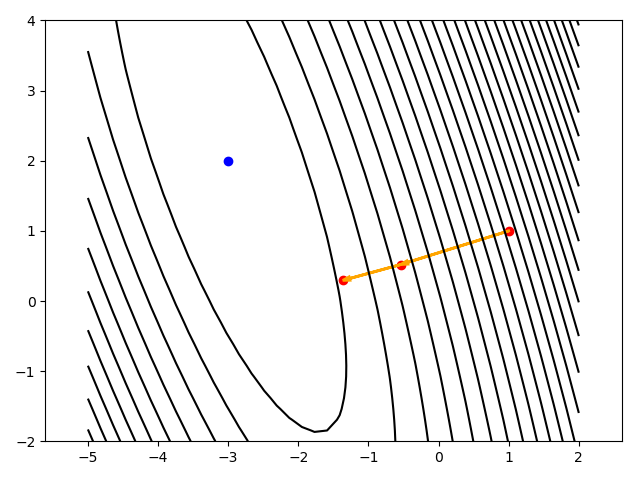
\includegraphics[scale=\myscale,scale=0.45]{figures/descente_pas_stochastique}
\end{center}
\end{minipage}
\begin{minipage}{0.48\textwidth}
\begin{center}
{\bf Descente de gradient stochastique}
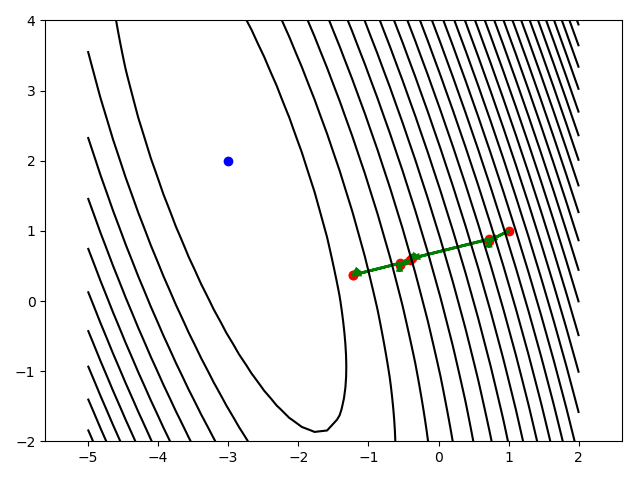
\includegraphics[scale=\myscale,scale=0.45]{figures/descente_stochastique}
\end{center}
\end{minipage}
\end{center}


Conclusion: sur cet exemple les points sont exactement sur la parabole d'équation $y=x^2+ax+b$ avec $a=-3$ et $b=2$. Bien sûr cette méthode est encore plus intéressante lorsqu'il s'agit de trouver une parabole qui ne contient pas l'ensemble des points donnés.
\myfigure{1}{
\tikzinput{fig-stochastique-02}
}

\end{exemple}




Terminons par des remarques plus techniques.
Tout d'abord, la formule précise de la descente de gradient stochastique est :
$$P_{k+1} = P_k - \delta \grad E_{(k \% N)+1} (P_k)$$
où $k \% N$ est \og{}$k$ modulo $N$\fg{}.



La descente de gradient stochastique est une méthode qui peut être plus efficace : 
\begin{itemize}
  \item Tout d'abord elle n'utilise qu'une donnée à la fois et évite ainsi les problèmes de mémoire de la descente classique pour laquelle il faut manipuler toutes les données à chaque itération.
  \item Toujours dans le cas où l'on a beaucoup de données, la descente de gradient stochastique peut converger en deux ou trois passages sur l'ensemble des données, alors que la descente classique nécessite toujours plusieurs itérations (voir la section \ref{ssec:lot} plus loin).
  \item Avec la méthode stochastique, on calcule des gradients en des points qui sont plus proches du minimum. Attention cependant, certains petits pas peuvent aller dans la mauvaise direction.
  \item Le caractère aléatoire de ces petits pas est parfois un avantage, par exemple pour s'échapper d'un point-selle.
\end{itemize}






%--------------------------------------------------------------------
\subsection{Différentes fonctions d'erreurs}

Il existe différentes formules pour calculer l'erreur entre la sortie attendue $y_i$ et la sortie produite $F(x_i)$.

On considère une série de valeurs $y_i$, $i=1,\ldots,N$ (fournie par observations ou expérimentations) qui sont approchées par des valeurs $F(x_i)$ produites par une formule issue d'un réseau de neurones par exemple.
Le but est d'obtenir $F(x_i)$ le plus proche possible de $y_i$, pour tout $i=1,\ldots,N$. Pour savoir si l'objectif est atteint, on mesure l'écart entre ces valeurs.

\textbf{Erreur quadratique moyenne.}
$$E = \frac{1}{N} \sum_{i=1}^N (y_i-F(x_i))^2.$$

C'est la formule la plus classique (en anglais \emph{minimal squared error} ou \emph{mse}). 
Bien entendu $E\ge0$ quels que soit les $F(x_i)$ et $E=0$ si et seulement si $y_i=F(x_i)$ pour tous les $i=1,\ldots,N$. 
C'est presque la formule que l'on a utilisée pour la régression linéaire (il n'y avait pas le facteur $\frac1N$).

\textbf{Erreur absolue moyenne.}
$$E = \frac{1}{N} \sum_{i=1}^N |y_i-F(x_i)|.$$

C'est une formule plus naturelle, mais moins agréable à manipuler à cause de la valeur absolue.

Noter que pour ces deux formules, l'erreur globale $E$ est la moyenne d'erreurs locales $E_i = (y_i-F(x_i))^2$ (ou bien $E_i = |y_i-F(x_i)|$).
Les erreurs locales sont indépendantes les unes des autres, ce qui est la base de la descente de gradient stochastique.
(Une formule d'erreur du type $E = y_1y_2 - F(x_1)F(x_2)$ ne permettrait pas la descente stochastique.)

Il existe d'autres formules d'erreur, en particulier si la sortie attendue est du type $0$ ou $1$ ou bien si la sortie produite est une probabilité $0\le p \le 1$. 

% [[Ces formules seront détaillées dans la partie \og{}Statistique et probabilités\fg{}.]]

%--------------------------------------------------------------------
\subsection{Descente par lots}
\label{ssec:lot}

\index{descente de gradient!par lots}

Il existe une méthode intermédiaire entre la descente de gradient classique (qui tient compte de toutes les données à chaque itération)
et la descente de gradient stochastique (qui n'utilise qu'une seule donnée à chaque itération).

La descente de gradient par \defi{lots} (ou \defi{mini-lots}, \emph{mini-batch}) est une méthode intermédiaire : on divise les données par paquets de taille $K$. Pour chaque paquet (appelé \og{}lot\fg{}), on calcule un gradient et on effectue une itération.

Au bout de $N/K$ itérations, on a parcouru tout le jeu de données : cela s'appelle une \defi{époque}.
\index{descente de gradient!epoque@époque}


\myfigure{1.2}{
\tikzinput{fig-epoque}
}

La formule est donc
$$P_{k+1} = P_k - \delta \grad (E_{j_0+1}+E_{j_0+2}+\cdots+E_{j_0+K}) (P_k).$$
Pour $P_{k+2}$, on repart de $P_{k+1}$ et on utilise le gradient de la fonction $E_{j_0+K+1}+E_{j_0+K+2}+\cdots+E_{j_0+2K}$.


\begin{remarque*}
\sauteligne
\begin{itemize}
  \item Pour $K=1$, c'est exactement la descente de gradient stochastique. Pour $K=N$, c'est la descente de gradient classique.
  
  \item Cette méthode combine le meilleur des deux mondes : la taille des données utilisées à chaque itération peut être adaptée à la mémoire et le fait de travailler par lots évite les pas erratiques de la descente stochastique pure.
  
  \item On peut par exemple choisir $2 \le K \le 32$ et profiter du calcul parallèle en calculant $\grad (E_1+\cdots + E_K)$, par le calcul de chacun des $\grad E_i$ sur $K$ processeurs, puis en additionnant les résultats.
  
  \item Il est d'usage de mélanger au hasard les données $(X_i,y_i)$ avant chaque époque.
\end{itemize}
\end{remarque*}



\begin{exemple}
Voyons un exemple d'interpolation circulaire.
Les $6$ points ci-dessous sont sur un cercle. Comment déterminer son centre et son rayon ?
\begin{center}
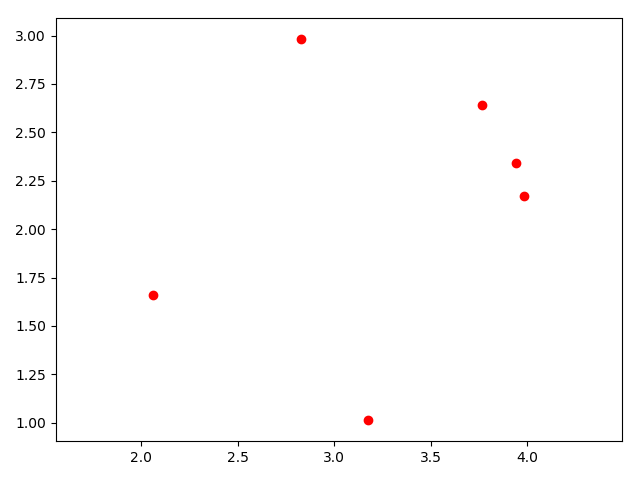
\includegraphics[scale=\myscale,scale=0.5]{figures/circulaire-01}
\end{center}

Pour des points $(x_i,y_i)$, $i=1,\ldots, N$, on mesure la distance globale par rapport au cercle $\mathcal{C}$ de centre $(a,b)$ et de rayon $c$ par la formule d'erreur :
$$E(a,b,c) = \sum_{i=1}^N E_i(a,b,c)$$
où 
$$E_i(a,b,c) = \big( (x_i-a)^2 + (y_i-b)^2 - c^2 \big)^2.$$
En effet, $E_i$ mesure en quelque sorte la distance entre le point $(x_i,y_i)$ et le cercle $\mathcal{C}$ de centre $(a,b)$ et de rayon $c$. Donc $E_i=0$ si et seulement si $(x_i,y_i) \in \mathcal{C}$, sinon $E_i > 0$.

\myfigure{1}{
\tikzinput{fig-circulaire-01}
}

Dans notre exemple, les $N = 6$ points sont exactement situés sur le cercle de centre $(a,b)$ et de rayon $c$. En appliquant la descente de gradient par lots avec $\delta = 0.01$ et $(a_0,b_0,c_0) = (1,1,2)$, on trouve $(a,b) = (3,2)$ et $c=1$.
Ci-dessous, à droite, nous avons représenté les valeurs de l'erreur totale $E$ (qui tend vers $0$) en fonction du nombre d'époques et ceci pour différentes tailles du lot : $K=1$ (descente stochastique), $K=2$, $K=3$ et $K=6$ (descente classique).
\begin{center}
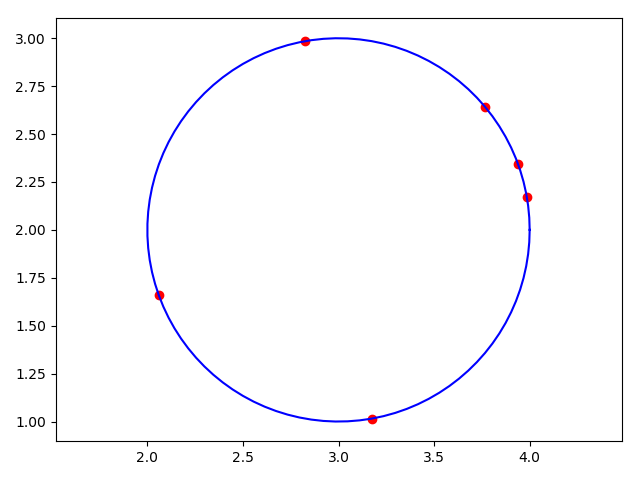
\includegraphics[scale=\myscale,scale=0.5]{figures/circulaire-02}
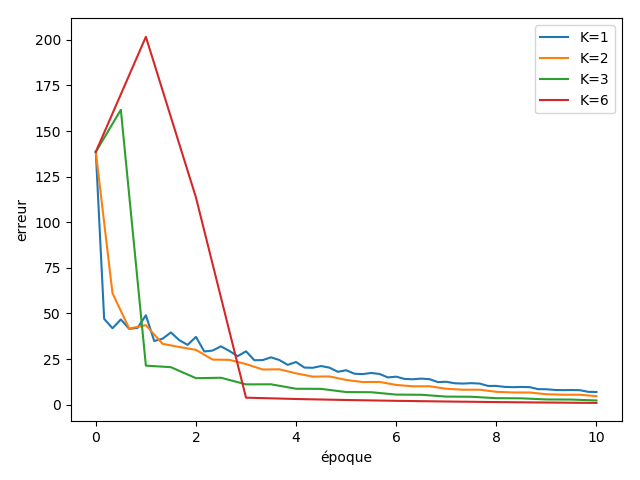
\includegraphics[scale=\myscale,scale=0.5]{figures/circulaire-03}
\end{center}
On remarque qu'au bout de $10$ époques la valeur de l'erreur est à peu près la même quelle que soit la taille $K$ de l'échantillon. Par contre, l'évolution au départ est différente. Par exemple pour $K=1$, l'erreur fluctue à la hausse ou à la baisse à chaque itération. 

Cette méthode présente bien sûr davantage d'intérêt quand les points ne sont pas exactement sur un cercle. Il s'agit alors de trouver le meilleur cercle qui convient, c'est-à-dire de trouver le minimum (cette fois non nul) de $E$.
Voici un exemple de $N = 100$ points tirés au hasard autour du cercle de centre $(a,b) = (1,2)$ et de rayon $c=3$.
La descente de gradient est appliquée avec $\delta = 0.001$ et $(a_0,b_0,c_0) = (1,1,1)$ pour des lots de différentes tailles $K=1$, $K=10$ et $K=20$. On remarque que deux époques suffisent pour avoir convergence et que plus la taille $K$ de l'échantillon est grande plus la convergence est régulière vers le minimum.

\begin{center}
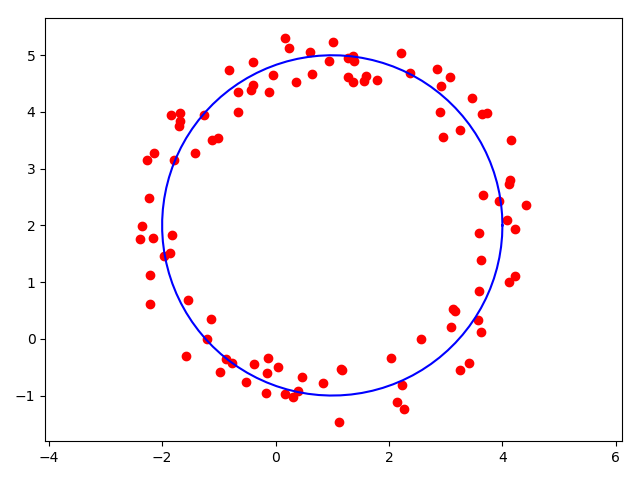
\includegraphics[scale=\myscale,scale=0.5]{figures/circulaire-04}
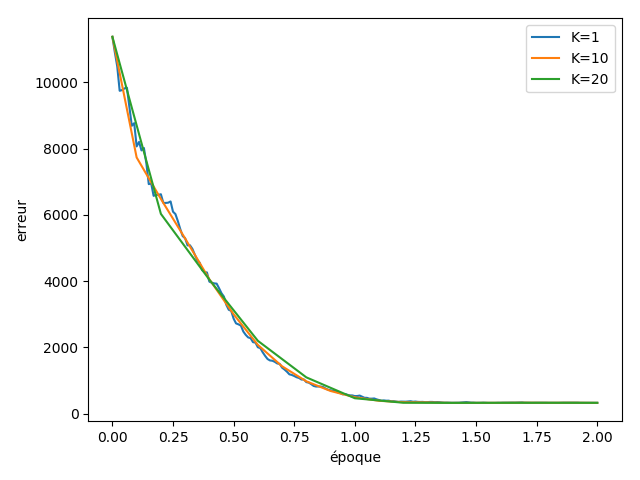
\includegraphics[scale=\myscale,scale=0.5]{figures/circulaire-05}
\end{center}

\end{exemple}

%%%%%%%%%%%%%%%%%%%%%%%%%%%%%%%%%%%%%%%%%%%%%%%%%%%%%%%%%%%%%%%%%%%%%
\section{Accélérations}


Le choix du pas $\delta$ n'est pas la seule amélioration possible de la méthode du gradient, nous allons voir comment la modifier à l'aide du \og{}moment\fg{}. Commençons par revenir à l'analogie de la descente du gradient classique qui correspond à une goutte d'eau qui descend une montagne : la goutte emprunte le chemin qui suit la courbe de plus grande pente, quitte à serpenter et osciller lors de la descente. Imaginons que l'on lance maintenant une balle assez lourde du haut de la même montagne. Cette balle va suivre, comme la goutte d'eau, le chemin de la plus forte pente, mais une fois lancée elle va acquérir de l'inertie, appelée \defi{moment}, qui va atténuer ses changements de direction.
Ainsi la balle ne s'embarrasse pas des petits aléas du terrain et dévale la pente plus rapidement que la goutte d'eau.


Nos petits aléas de terrain à nous viennent du fait que l'on ne calcule pas exactement le gradient de la fonction d'erreur en utilisant tout le jeu de données à chaque fois, mais seulement un échantillon. Cela peut conduire à certains gradients mal orientés. L'inertie de la balle est en quelque sorte la mémoire de la trajectoire passée qui corrige les mouvements erratiques.

Sur la figure de gauche, la descente classique (la goutte d'eau), sur la figure de droite, la descente de gradient avec le moment (la balle).

\myfigure{1}{
\tikzinput{fig_moment01}\qquad\qquad 
\tikzinput{fig_moment02}
}

%--------------------------------------------------------------------
\subsection{Moment}

\index{descente de gradient!moment}

Rappelons la formule de la descente de gradient classique :
$$P_{k+1} = P_k - \delta \grad f(P_k).$$

\myfigure{1}{
\tikzinput{fig_moment03}
}

Considérons nos points comme une particule qui voyage au cours du temps. Alors
le vecteur $\overrightarrow{P_{k-1}P_k}$ correspond à la vitesse de cette particule et est appelé le \defi{moment} au point $P_k$.

La formule de la descente de gradient avec moment est :
$$P_{k+1} = P_k + \mu\overrightarrow{P_{k-1}P_k}  - \delta \grad f(P_k).$$
où $\mu,\delta \in \Rr$. Cette formule peut être définie pour $k=0$ si on suppose que la particule est immobile au départ, c'est-à-dire en posant $\overrightarrow{P_{-1}P_0} = \vec 0$.

On peut prendre par exemple $\mu \in [0.5,0.9]$ et $\delta = 0.01$.


Schématiquement, au point $P_k$ nous avons deux vecteurs : un qui provient du moment $\mu\overrightarrow{P_{k-1}P_k}$ (la mémoire du passé) et un qui provient du gradient $- \delta \grad f(P_k)$ (qui projette vers l'avenir). La somme permet de calculer le point suivant  $P_{k+1}$.

\myfigure{1.2}{
\tikzinput{fig_moment04}
}





%--------------------------------------------------------------------
\subsection{Nesterov}

\index{descente de gradient!acceleration de Nesterov@accélération de Nesterov}

Dans la méthode précédente, le moment et le gradient sont calculés au même point $P_k$. La méthode de Nesterov est une variante de cette méthode. 
Elle consiste à appliquer d'abord le moment, pour obtenir un point $P_k'$, puis de calculer le gradient en ce point (et non en $P_k$).

La formule est donc 
$$P_{k+1} = P_k + \mu\overrightarrow{P_{k-1}P_k}  - \delta \grad f(P_k+\mu\overrightarrow{P_{k-1}P_k}).$$
Autrement dit, si on note $P_k'$ le point $P_k + \mu\overrightarrow{P_{k-1}P_k}$ alors
$$P_{k+1} = P_k'  - \delta \grad f(P_k').$$

\myfigure{1.2}{
\tikzinput{fig_moment05}
}


C'est un petit avantage par rapport à la méthode du moment puisqu'on calcule le gradient au point $P_k'$ qui est censé être plus près de la solution $P_{\min}$ que $P_k$.


%--------------------------------------------------------------------
\subsection{Vocabulaire}

Terminons par un petit résumé du vocabulaire avec sa traduction en anglais :
\begin{itemize}
 \item descente de gradient (classique), \emph{(batch) gradient descent},
 \item descente de gradient stochastique, \emph{sgd} pour \emph{stochastic gradient descent},
 \item descente de gradient par lots, \emph{mini-batch gradient descent},
 \item pas $\delta$, \emph{learning rate},
 \item erreur quadratique moyenne, \emph{mse} pour \emph{minimal squared error},
 \item moment, \emph{momentum},
 \item époque, \emph{epoch}.
 \end{itemize}  


\end{document}
